% !TeX root = ./Serie03-JoelZuber-YannikDaellenbach.tex
% Analysieren Sie mit Hilfe eines STN einen Benutzer-System-Dialog 
% auf einer Webseite oder einer Applikation auf einem technischen Gerät (z.B. einem Smartphone o.ä.). 
% Untersuchen Sie nur einen bestimmten Aspekt des Dialoges, z.B.
% - Neuen Kontakt zum Adressbuch hinzufügen (oder einen bestehenden Kontakt bearbeiten oder löschen)
% - Im Kalender ein neues Ereignis hinzufügen (oder ein bestehendes Ereignis bearbeiten oder löschen)
% - Auf einer Webseite ein Benutzerkonto eröffnen und wieder löschen
% - Einen Artikel zum Warenkorb eines Webshops hinzufügen (oder einen Warenkorb modifizieren oder löschen)
%
% Versuchen Sie ein möglichst interessantes Beispiel zu finden, das ein Problem aufdeckt. 
% Mögliche Probleme könnten sein:
% - Ein gefährlicher Zustand/Übergang wird nicht genügend gut als solcher markiert (z.B. wenn ein Datenverlust droht).
% - Ein unerwünschter Zustand kann nicht schrittweise rückgängig gemacht werden.
% - Eine bestimmte Operation ist nur mit viel Aufwand wieder umkehrbar.
% - Die Anwendung einer nicht vorgesehenen Aktion in einem bestimmten Zustand führt zu einem ungewöhnlichen Verhalten des Systems.
% - etc.
\textbf{Problem:} Es muss immer ein vertrauenswürdiges Gerät registriert sein. 
Wer sein letztes vertrauenswürdiges Gerät verliert, kann sich nicht anmelden und ein neues Gerät registrieren. 
Ein theoretisch möglicher Zustand ist nicht erreichbar.
\begin{figure}[H]
  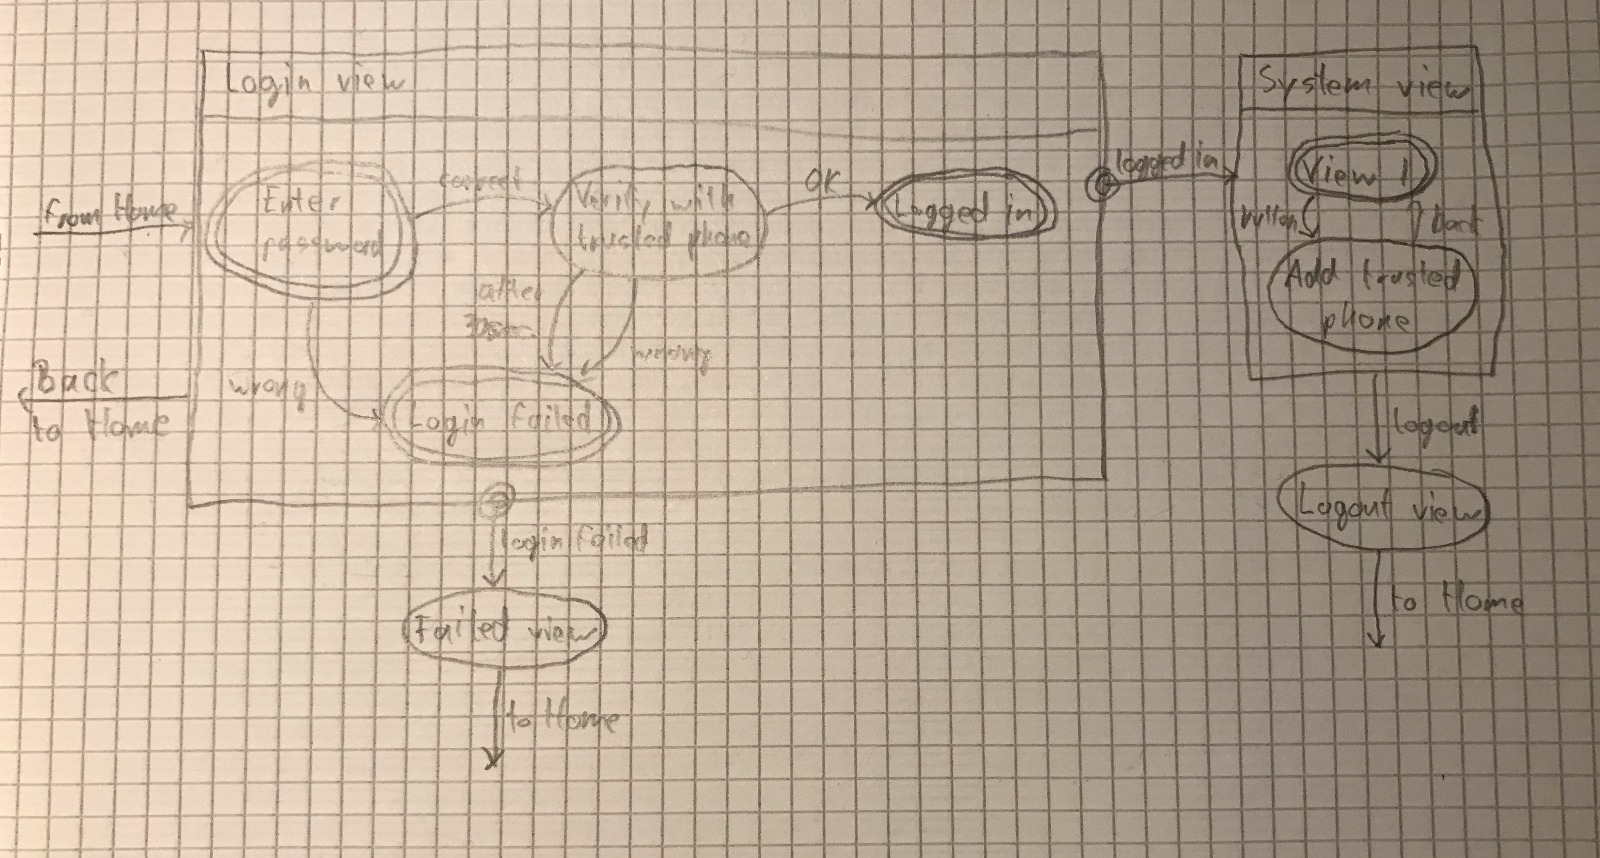
\includegraphics[width=\textwidth]{data/STN_Login.jpeg}
  \caption{Beispiel Login WKB (STN stark vereinfacht)}
\end{figure}